\documentclass[tikz,border=4pt]{standalone}
\usepackage{tikz}
\usepackage{amsmath}
\usetikzlibrary{arrows.meta,decorations.pathreplacing,positioning}

\begin{document}
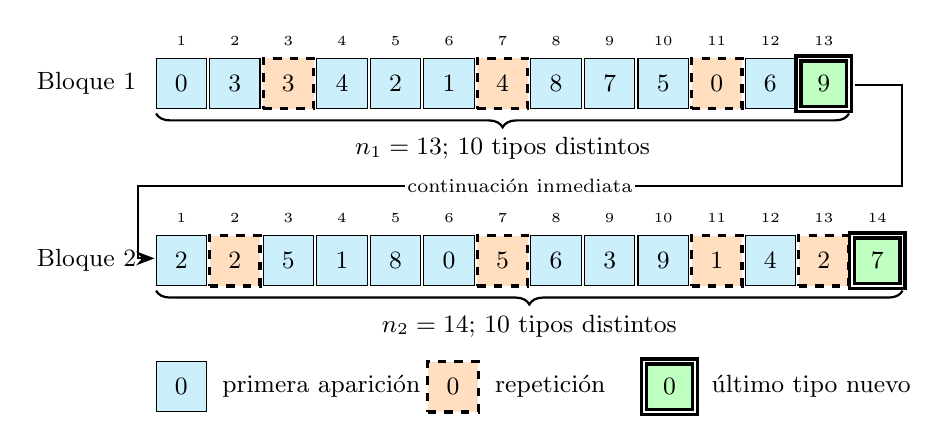
\begin{tikzpicture}[
    cell/.style={draw=black,minimum width=6.4mm,minimum height=6.4mm,
        inner sep=0pt,font=\small},
    first/.style={cell,fill=cyan!20},
    repeated/.style={cell,fill=orange!25,dashed,very thick},
    completing/.style={cell,fill=green!25,double,very thick},
    label/.style={font=\small}
]
    \def\step{0.68}

    \node[label,anchor=east] at (-0.45,3) {Bloque 1};
    \foreach \pos/\digit/\kind in {
        1/0/first,2/3/first,3/3/repeated,4/4/first,5/2/first,
        6/1/first,7/4/repeated,8/8/first,9/7/first,10/5/first,
        11/0/repeated,12/6/first,13/9/completing} {
        \pgfmathsetmacro{\x}{(\pos-1)*\step}
        \node[\kind] at (\x,3) {\digit};
        \node[font=\tiny,above=1pt] at (\x,3.32) {\pos};
    }
    \draw[decorate,decoration={brace,amplitude=5pt,mirror},thick]
        (-0.32,2.62) -- (8.48,2.62)
        node[midway,below=5pt,label] {$n_1=13$; 10 tipos distintos};

    \draw[-{Stealth},thick] (8.55,2.98) -- (9.15,2.98) -- (9.15,1.70)
        -- (-0.55,1.70) -- (-0.55,0.78) -- (-0.34,0.78);
    \node[fill=white,inner sep=1pt,font=\scriptsize] at (4.3,1.70)
        {continuación inmediata};

    \node[label,anchor=east] at (-0.45,0.75) {Bloque 2};
    \foreach \pos/\digit/\kind in {
        1/2/first,2/2/repeated,3/5/first,4/1/first,5/8/first,
        6/0/first,7/5/repeated,8/6/first,9/3/first,10/9/first,
        11/1/repeated,12/4/first,13/2/repeated,14/7/completing} {
        \pgfmathsetmacro{\x}{(\pos-1)*\step}
        \node[\kind] at (\x,0.75) {\digit};
        \node[font=\tiny,above=1pt] at (\x,1.07) {\pos};
    }
    \draw[decorate,decoration={brace,amplitude=5pt,mirror},thick]
        (-0.32,0.37) -- (9.16,0.37)
        node[midway,below=5pt,label] {$n_2=14$; 10 tipos distintos};

    \node[first] (legend-first) at (0,-0.85) {0};
    \node[label,right=2pt of legend-first] {primera aparición};
    \node[repeated] (legend-repeat) at (3.45,-0.85) {0};
    \node[label,right=2pt of legend-repeat] {repetición};
    \node[completing] (legend-complete) at (6.2,-0.85) {0};
    \node[label,right=2pt of legend-complete] {último tipo nuevo};

\end{tikzpicture}
\end{document}
